\begin{task}{4, Time-delay embedding}
In this task we will explore embeddings using time-delays, primarily based on Takens theorem. The functions used for this task can be found in \verb|utils.py|, being some of them the Lorenz system's functions used in Exercise 4. The experiments and the results for this task can be found in the notebook \verb|task4.ipynb|.

\paragraph{Part 1} Now, for this part of the task we will load the \verb|takens_1.txt| dataset and will work with it. This dataset contains a matrix \(X \in \mathbb{R}^{1000\times2}\) where the two columns of the matrix are the two coordinates of a closed, one-dimensional manifold. The visualization of the raw data can be observed in Figure \ref{takens_plot}.
\begin{figure}[H]
\centering
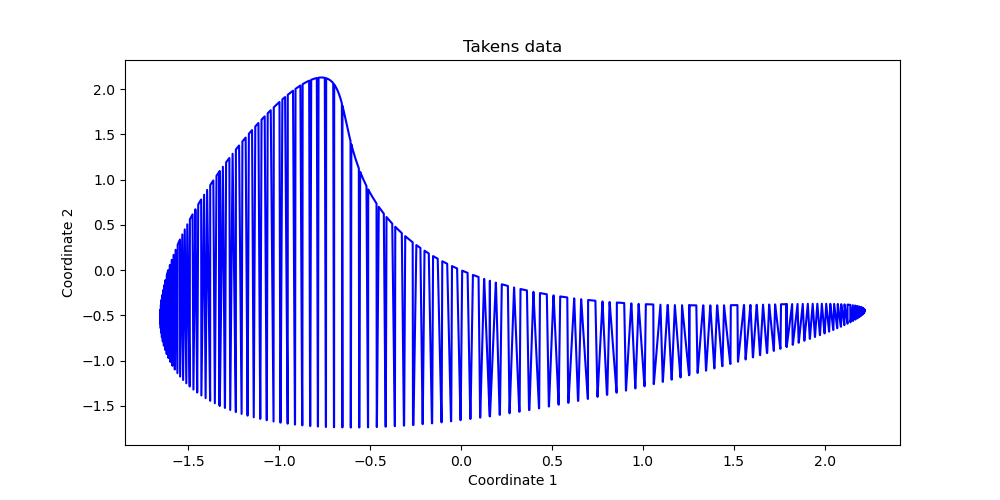
\includegraphics[width=0.7\textwidth]{images/takens_data.png}
\caption{Plotted dataset}
\label{takens_plot}
\end{figure}

Supposing that each row number represents "time," we can plot the first and second coordinates of the data against time (Figure \ref{takens_coor}).

\begin{figure}[H]
\centering
\subfigure[Coordinate 1 vs Time]{
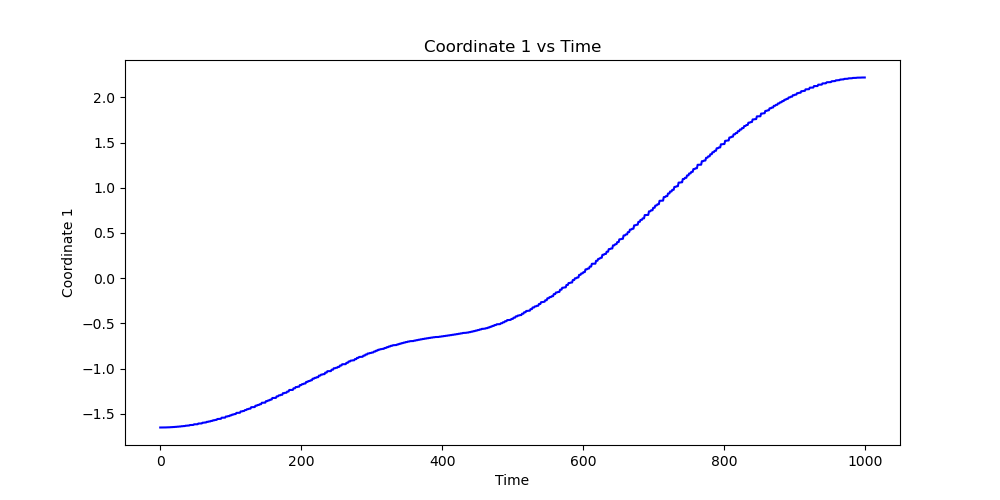
\includegraphics[width=0.5\textwidth]{images/takens_data_time.png}\label{takens_coora}}
\subfigure[Coordinate 2 vs Time]{
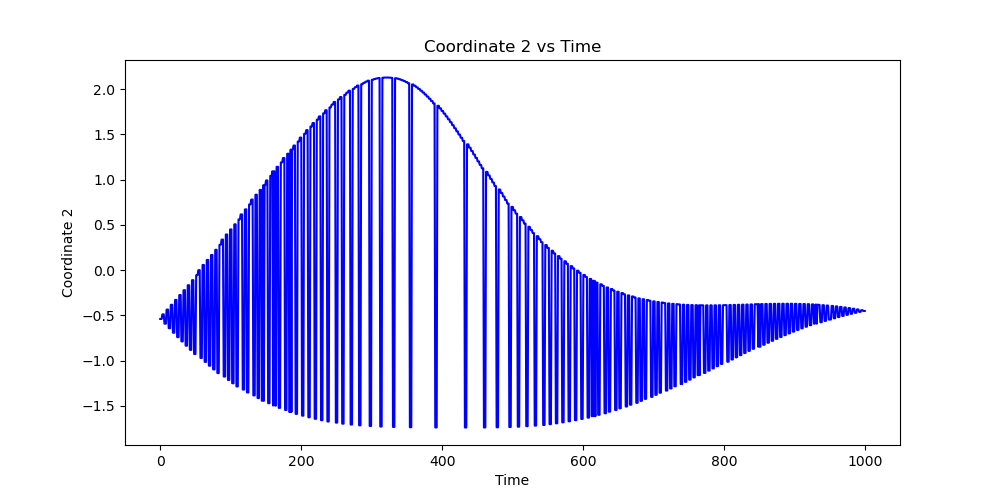
\includegraphics[width=0.5\textwidth]{images/takens_data_time2.png}\label{takens_coorb}}
\caption{Coordinates of the dataset against the row number (time)}
\label{takens_coor}
\end{figure}

However, in this task, we will focus on the first coordinate, i.e., Figure \ref{takens_coora}. Based on the Takens theorem, we will test some delays \(\Delta t\), equivalent to \(\Delta n\) rows in this case, to create an approximated version of an embedded representation of the original time series in a higher-dimensional space.


To generate delayed vectors, we employ the \verb|numpy.roll| function, facilitating the shift of array elements along a specified axis. This function seamlessly reintroduces elements that surpass the last position back to the initial position. Consequently, employing a roll of -1, equivalent to a delay of 1 row, results in the initial row of the original array occupying the final position in the delayed array. This behavior manifests as a sudden drop at the plot's conclusion, as illustrated in Figure \ref{coor_d1a}. To enhance the plot, the decision is made to exclude the last data points, as the information loss is negligible. This adjustment yields the improved plot depicted in Figure \ref{coor_d1b}. Additionally, to eliminate this drop from the plot for any value of \(delay\), it is necessary to skip the last \(delay\) data points, where \(delay \in \mathbb{N}\).

\begin{figure}[H]
\centering
\subfigure[Plotting the last point]{
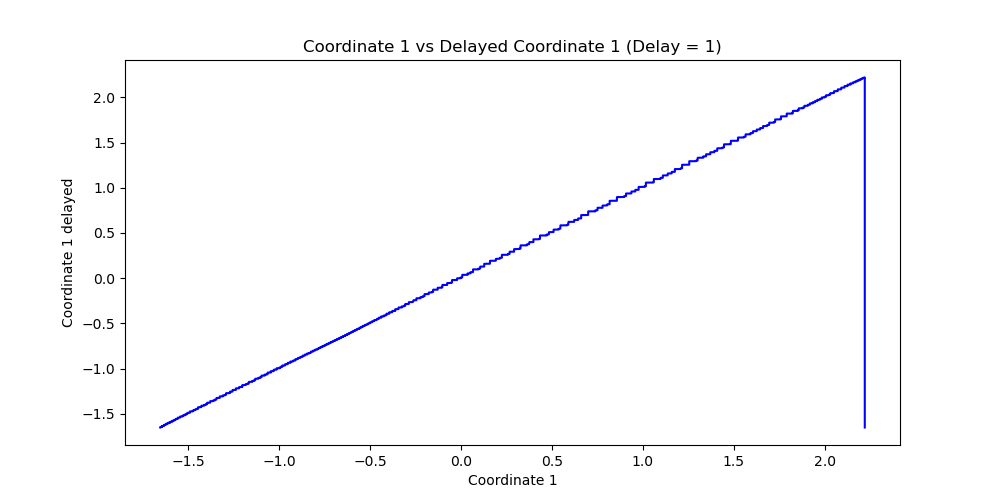
\includegraphics[width=0.5\textwidth]{images/takens_data_delay_w.png}\label{coor_d1a}}
\subfigure[Not plotting the last point]{
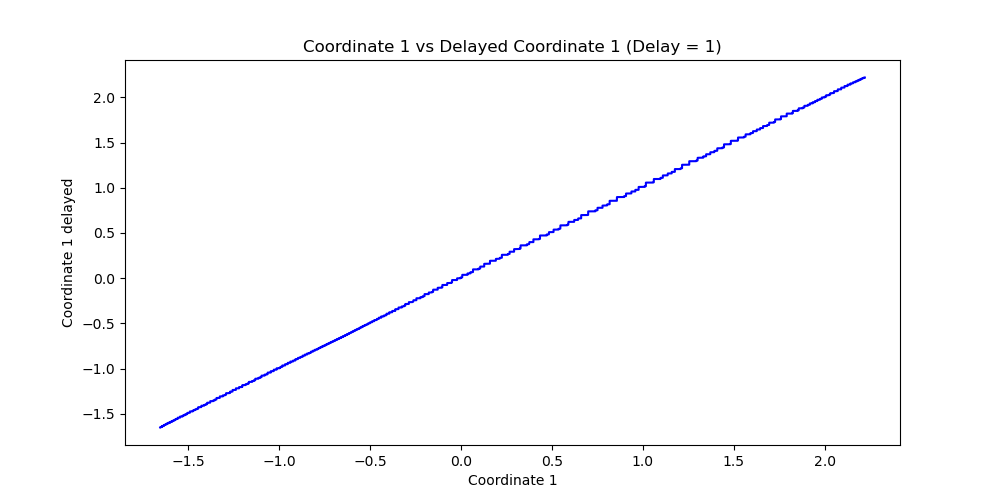
\includegraphics[width=0.5\textwidth]{images/takens_data_delay.png}\label{coor_d1b}}
\caption{Coordinate 1 against its delayed version (delay = 1)}
\label{coor_d1}
\end{figure}


We can observe in Figure \ref{coor_d1b} an increasing straight line, that suggests a strong linear correlation between each data point and its immediate successor in the time series. This pattern might indicate that the first coordinate is changing steadily with each subsequent data point. However, this line does not reveal too much of the underlying behaviour of the original first coordinate. We can try to increase the \(\Delta n\) to test how the increment of the delay changes the captured patterns in the system.
\begin{figure}[H]
\centering
\subfigure[Delay = 10]{
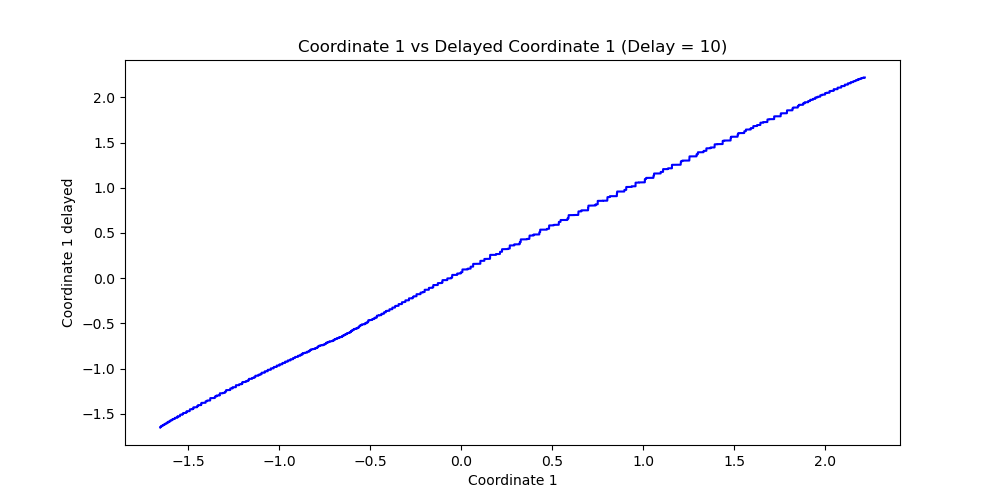
\includegraphics[width=0.45\textwidth]{images/takens_data_delay_10.png}\label{coor_d10a}}
\subfigure[Delay = 40]{
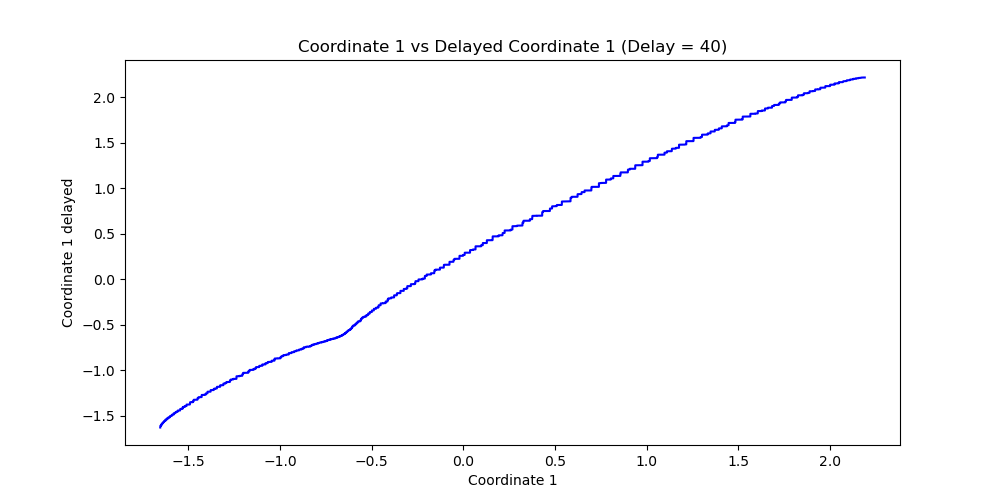
\includegraphics[width=0.45\textwidth]{images/takens_data_delay_40.png}\label{coor_d10b}}
\subfigure[Delay = 80]{
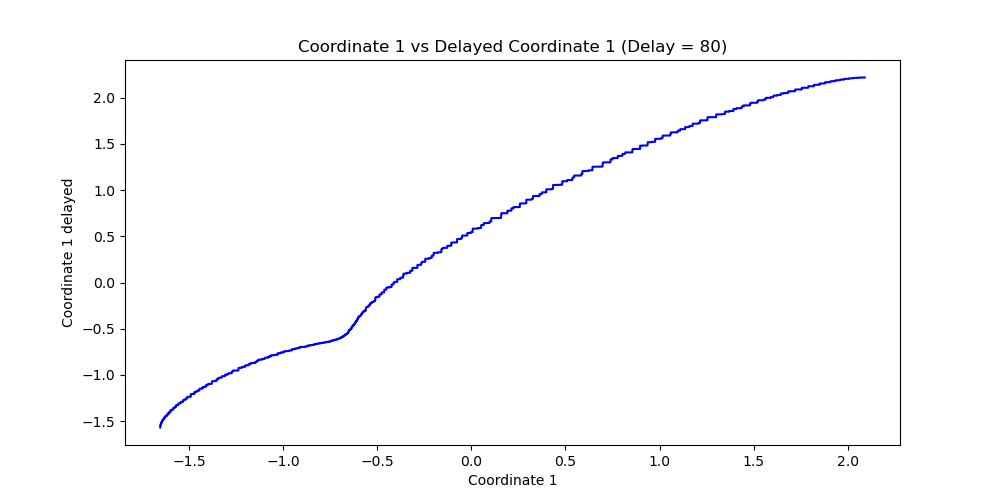
\includegraphics[width=0.45\textwidth]{images/takens_data_delay_80.png}\label{coor_d10c}}
\subfigure[Delay = 150]{
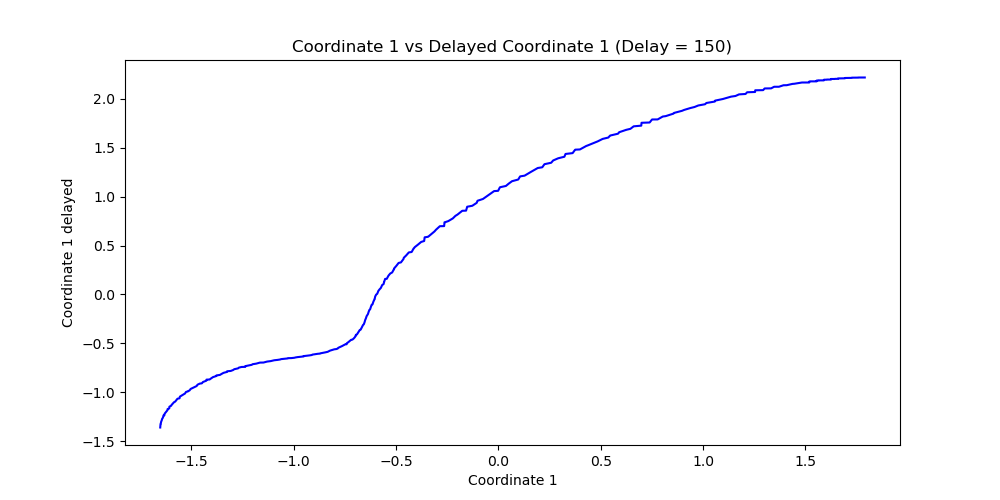
\includegraphics[width=0.45\textwidth]{images/takens_data_delay_150.png}\label{coor_d10d}}
\subfigure[Delay = 200]{
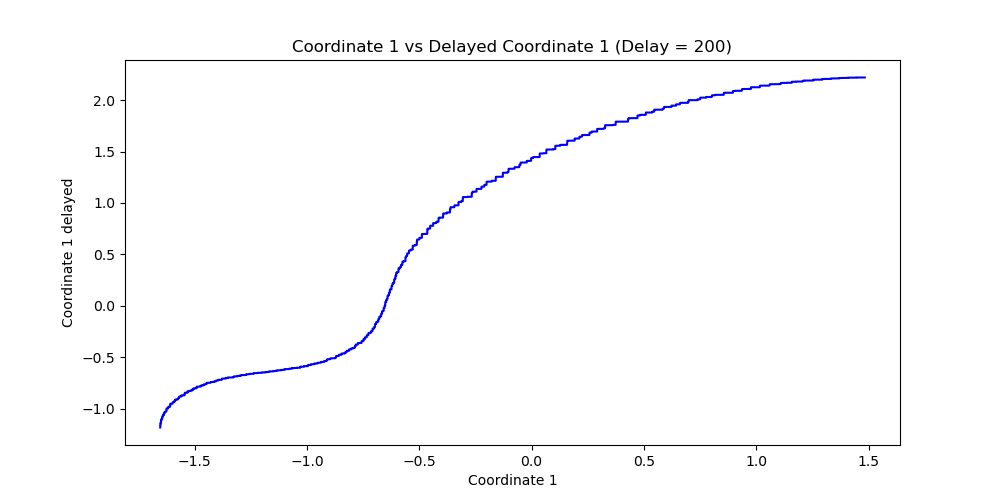
\includegraphics[width=0.45\textwidth]{images/takens_data_delay_200.png}\label{coor_d10e}}
\subfigure[Delay = 300]{
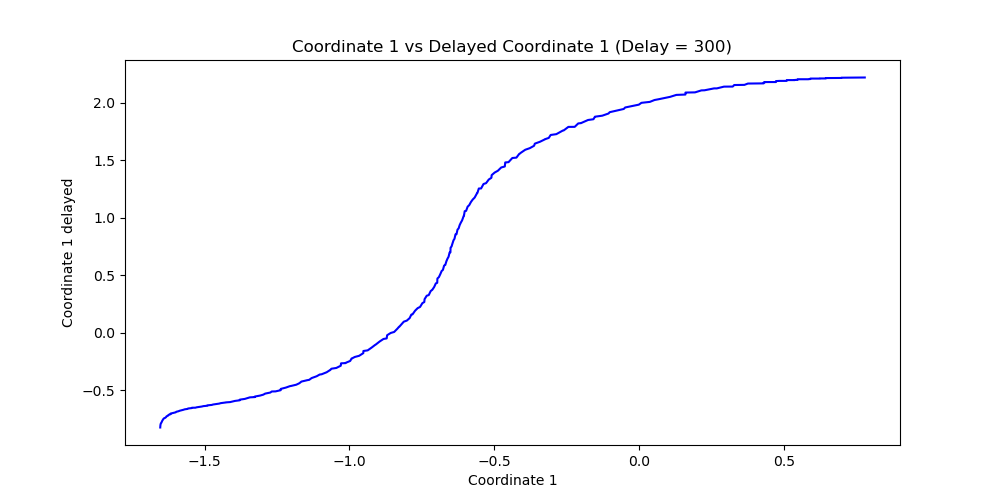
\includegraphics[width=0.45\textwidth]{images/takens_data_delay_300.png}\label{coor_d10f}}
\caption{Coordinate 1 against its delayed version for different delay values}
\label{coor_d10}
\end{figure}

Now, we analyze the plots generated for different delay values. In Figure \ref{coor_d10a}, where the delay is set to 10, the resulting graph maintains a straight line. Moving to delays of 40 and 80 (Figures \ref{coor_d10b}, \ref{coor_d10c} and \ref{coor_d10d}), curvature becomes evident, especially at the beginning. This observation suggests that these delays are more effective in capturing certain nonlinear features of the system, and the overall structure of the original first coordinate plot is adequately approximated, primarily for \(delay = 150\). However, delays of 200 and 300 (Figures \ref{coor_d10e} and \ref{coor_d10f}) introduce even more pronounced curvature. While this might capture additional complexities, it deviates from the original first coordinate plot, potentially introducing noise to the embedding. Additionally, using delays of 200 and 300 results in the loss of information as they involve plotting fewer points.

Takens' theorem states that we need \(2d + 1\) dimensions to faithfully embed the dynamics of a dynamical system with an intrinsic dimension \(d\) \cite{shalizi2006methods}. In other words, to capture the essential features and reconstruct the original system, the embedding space should have a dimension equal to or greater than \(2d + 1\), but it could be less in some scenarios \cite{baranski2020probabilistic}.

Therefore, in our case, being the dimension of the manifold \(d = 1\), we would need 3 dimensions to be sure that we embed the manifold correctly, making the dynamics of the system deterministic according to the theory. Thus, we have experimented using an embedding of 3 dimensions. We use the delay vector of the previous part as second coordinate and another delay vector which doubles the delay of the second coordinate, as the third coordinate.

\begin{figure}[H]
\centering
\subfigure[Delay = 1]{
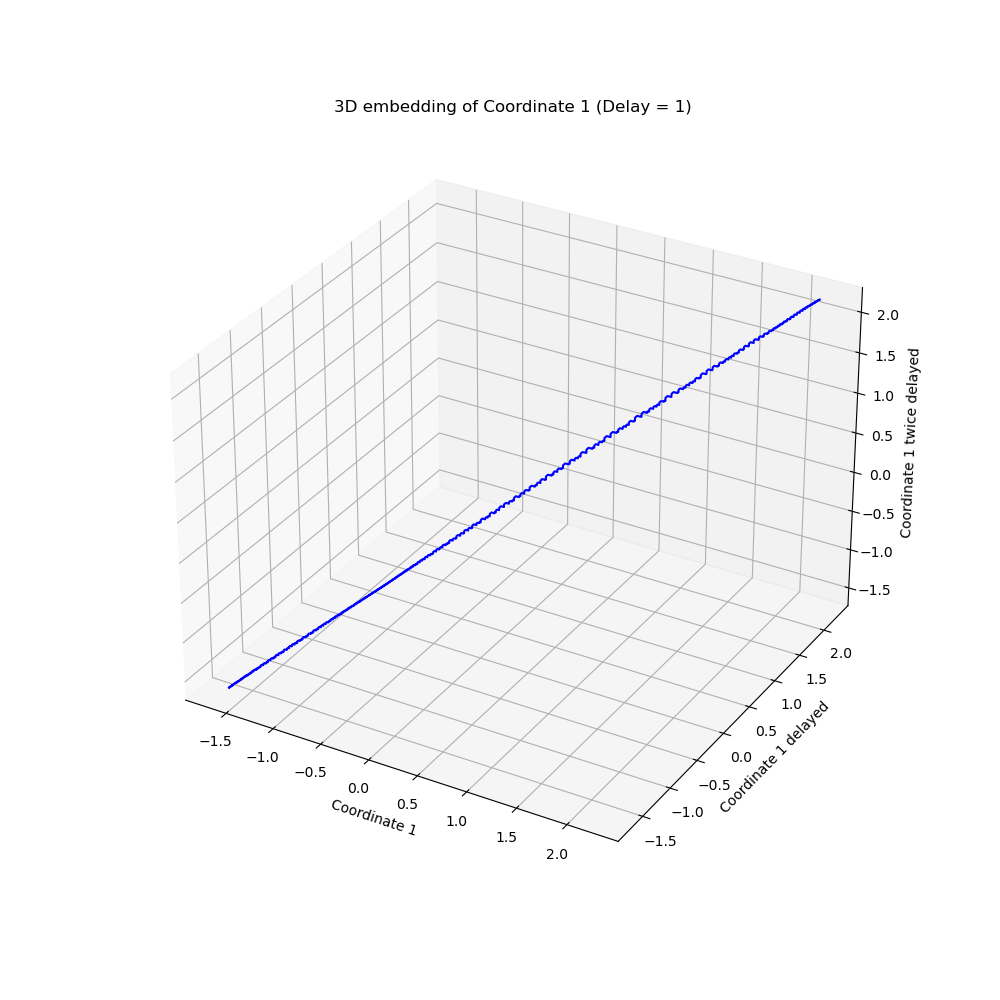
\includegraphics[width=0.45\textwidth]{images/takens_data_3D_1.png}\label{coor_d3da}}
\subfigure[Delay = 150]{
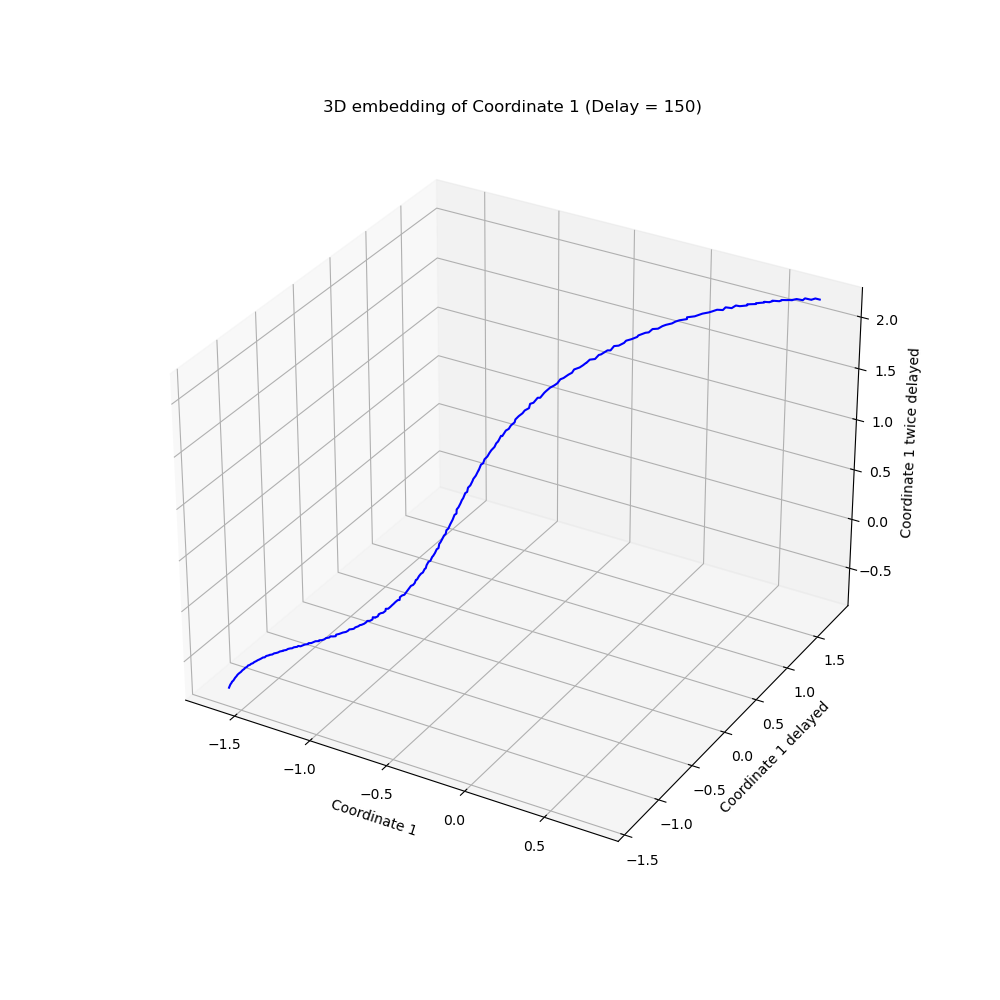
\includegraphics[width=0.45\textwidth]{images/takens_data_3D_150.png}\label{coor_d3db}}
\subfigure[Delay = 200]{
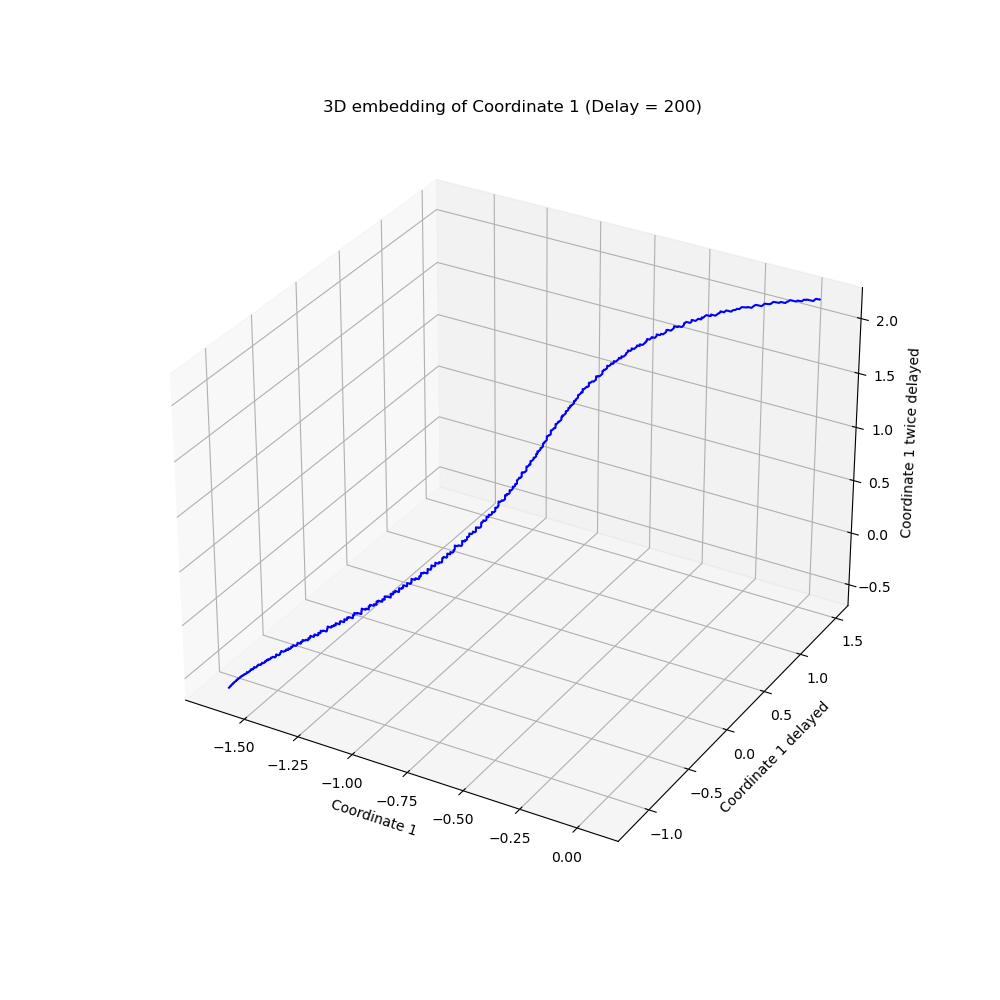
\includegraphics[width=0.45\textwidth]{images/takens_data_3D_200.png}\label{coor_d3dc}}
\subfigure[Delay = 300]{
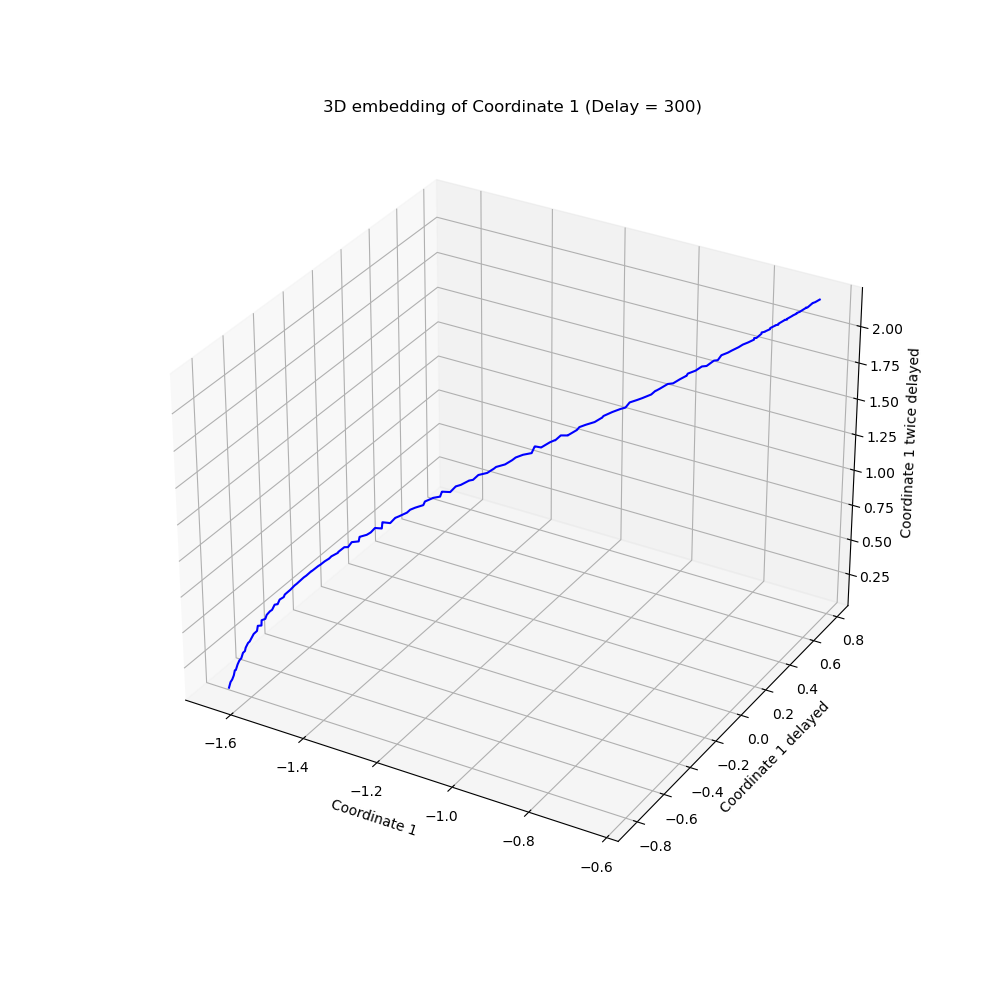
\includegraphics[width=0.45\textwidth]{images/takens_data_3D_300.png}\label{coor_d3dd}}
\caption{3D embedding of the system}
\label{coor_d3d}
\end{figure}

We can observe now how with \(delay = 1\) the obtained representation is still a straight line (Figure \ref{coor_d3da}). However, in Figures \ref{coor_d3db} and \ref{coor_d3dc} a more faithful approximation of the original structure is achieved. Finally, for a bigger delay in Figure \ref{coor_d3dd} the representation becomes less accurate due to the potential introduction of noise and miss of information, demonstrating the importance of selecting an appropriate delay parameter for the Takens embedding process.

Finally, for the sake of completeness we include additional figures that incorporate the last delay rows (Figure \ref{noskippart}). This enables us to better understand the approximation and test our assumption that excluding these rows from the plot does not significantly compromise the graphical representation of the overall structure, even with high delay values, as observed in Figure \ref{noskippartb}. For 3D plots the graphical representation is worsened and also does not provide much information about the overall structure as can be seen in Figure \ref{noskippartc}. In the next part, we will observe that, for more complex systems with greater amounts of data, omitting these rows becomes less critical for visualization, as their proportion in the plot is relatively smaller.
\begin{figure}[H]
\centering
\subfigure[Delay = 80]{
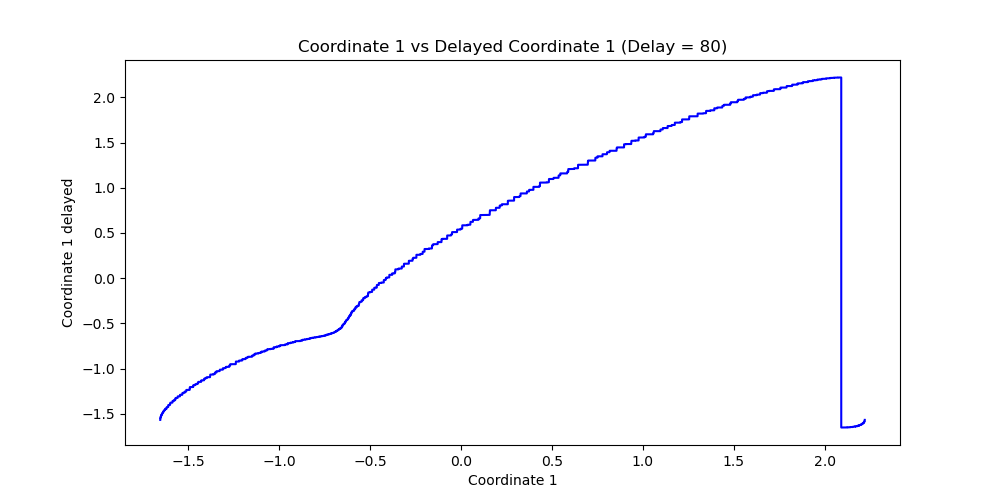
\includegraphics[width=0.45\textwidth]{images/takens_data_delay_80_noskip.png}\label{noskipparta}}
\subfigure[Delay = 200]{
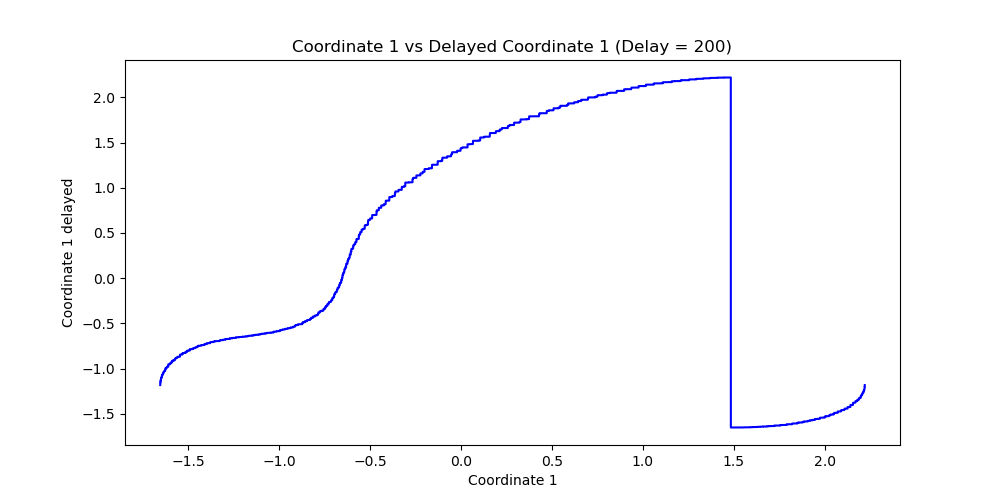
\includegraphics[width=0.45\textwidth]{images/takens_data_delay_200_noskip.png}\label{noskippartb}}
\subfigure[Delay = 50 3D Plot]{
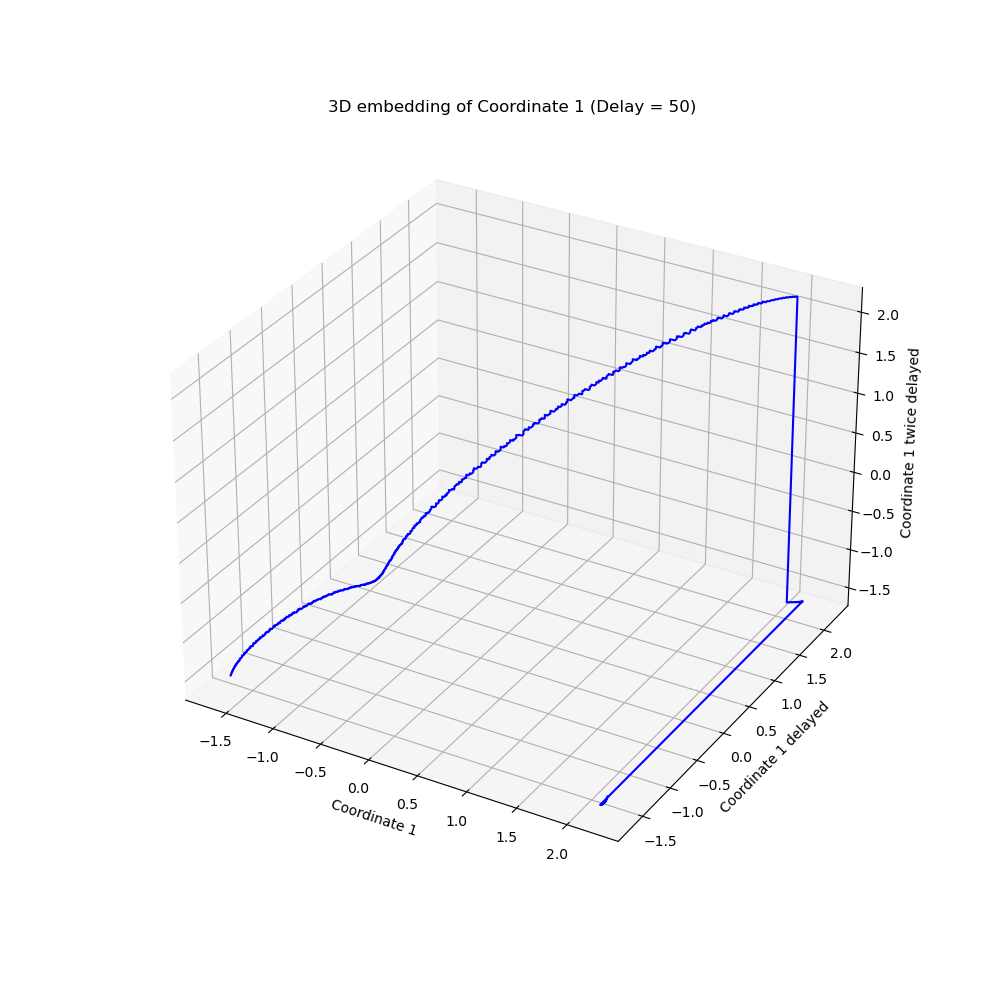
\includegraphics[width=0.45\textwidth]{images/takens_data_3D_50_noskip.png}\label{noskippartc}}
\subfigure[Delay = 200 3D Plot]{
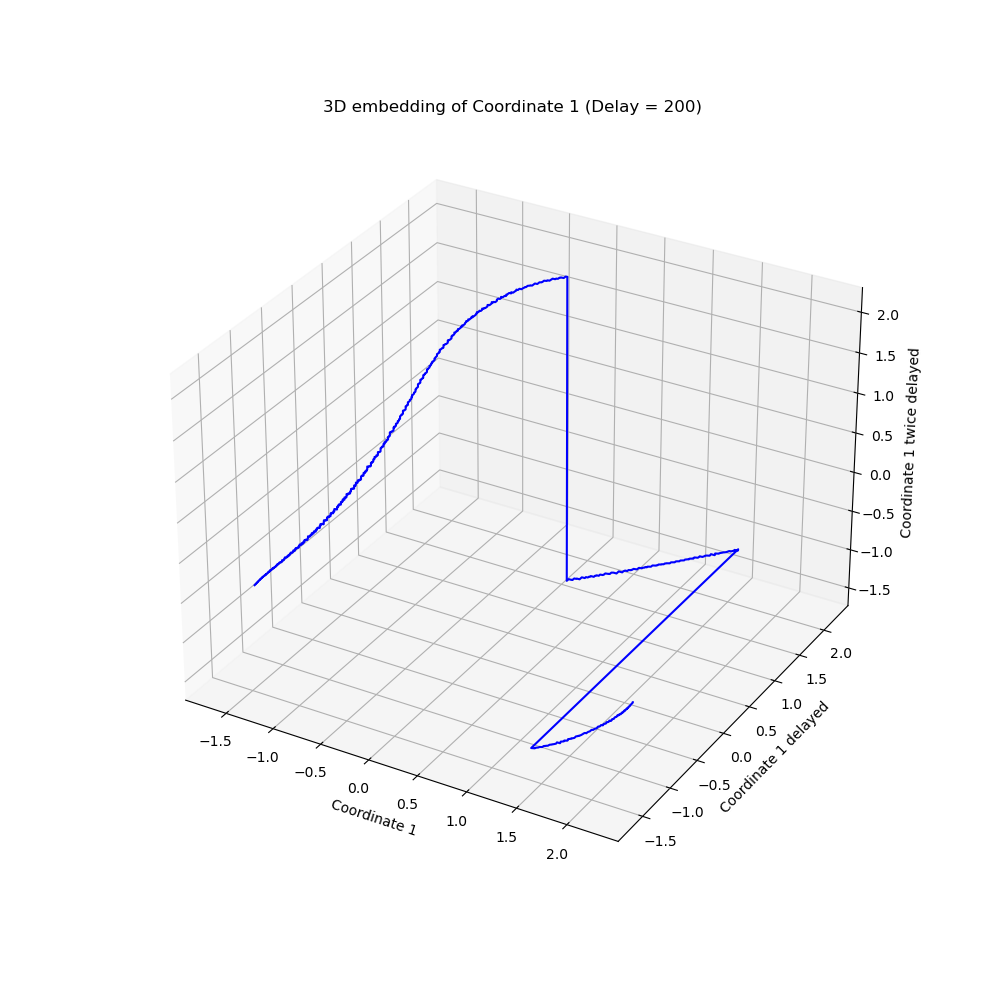
\includegraphics[width=0.45\textwidth]{images/takens_data_3D_200_noskip.png}\label{noskippartd}}
\caption{Plots without skipping the last \(delay\) rows}
\label{noskippart}
\end{figure}



\paragraph{Part 2} In this task, our objective is to approximate the chaotic dynamics of the Lorenz attractor using the Takens theorem. Since we have previously explored the Lorenz system in Exercise 4, we will skip providing an introduction and explanation of this system in the current task.

Assuming we only have access to the x-coordinate of the Lorenz system, our goal is to approximate the real system using a 3-dimensional space. According to the Takens theorem, this space enables us to obtain a reasonable understanding of the attractor's shape. The three dimensions in our space are represented by \(x_1 = x(t)\), \(x_2 = x(t + \Delta t)\), and \(x_3 = x(t + 2\Delta t)\), where \(t\) is a value greater than 0 that we need to choose.

Unlike the previous part, which was more exploratory, the aim here is to find a good approximation of the system given a 3-dimensional space.
Therefore, to select \(\Delta t\), we have implemented a function \verb|best_delay| inside \verb|utils.py|, instead of relying on visual inspection as done previously. This function determines the optimal \(\Delta t\) value that best approximates the system. The search for this optimal value is conducted within a specified range, limited to computational efficiency considerations (ranging from 1 to 100). The selection criterion is based on minimizing the distance between each point of the original trajectory and its corresponding point on the approximated trajectory, thus the closest approximation will be selected.

If we opt for a random selection of the delay \(\Delta t\) without using the selection algorithm, the results exhibit significant instability compared to the previous approach. This instability is likely attributed to the chaotic nature inherent in the system. In Figure \ref{lorenzdelaya}, the original structure is recognizable but appears flattened. However, in Figures \ref{lorenzdelayb} and \ref{lorenzdelayc}, the structure diverges considerably from the original. This observation aligns with our earlier findings in the previous exercise, where we found that the Lorenz attractor, under the given parameters, experiences a chaotic explosion in the distance between the original trajectory and a slightly perturbed one around \(t = 20\). Thus, attempting to approximate the system using a completely chaotic delayed version may result in an outcome that does not represent the correct trajectory.
\begin{figure}[H]
\centering
\subfigure[Delay = 1]{
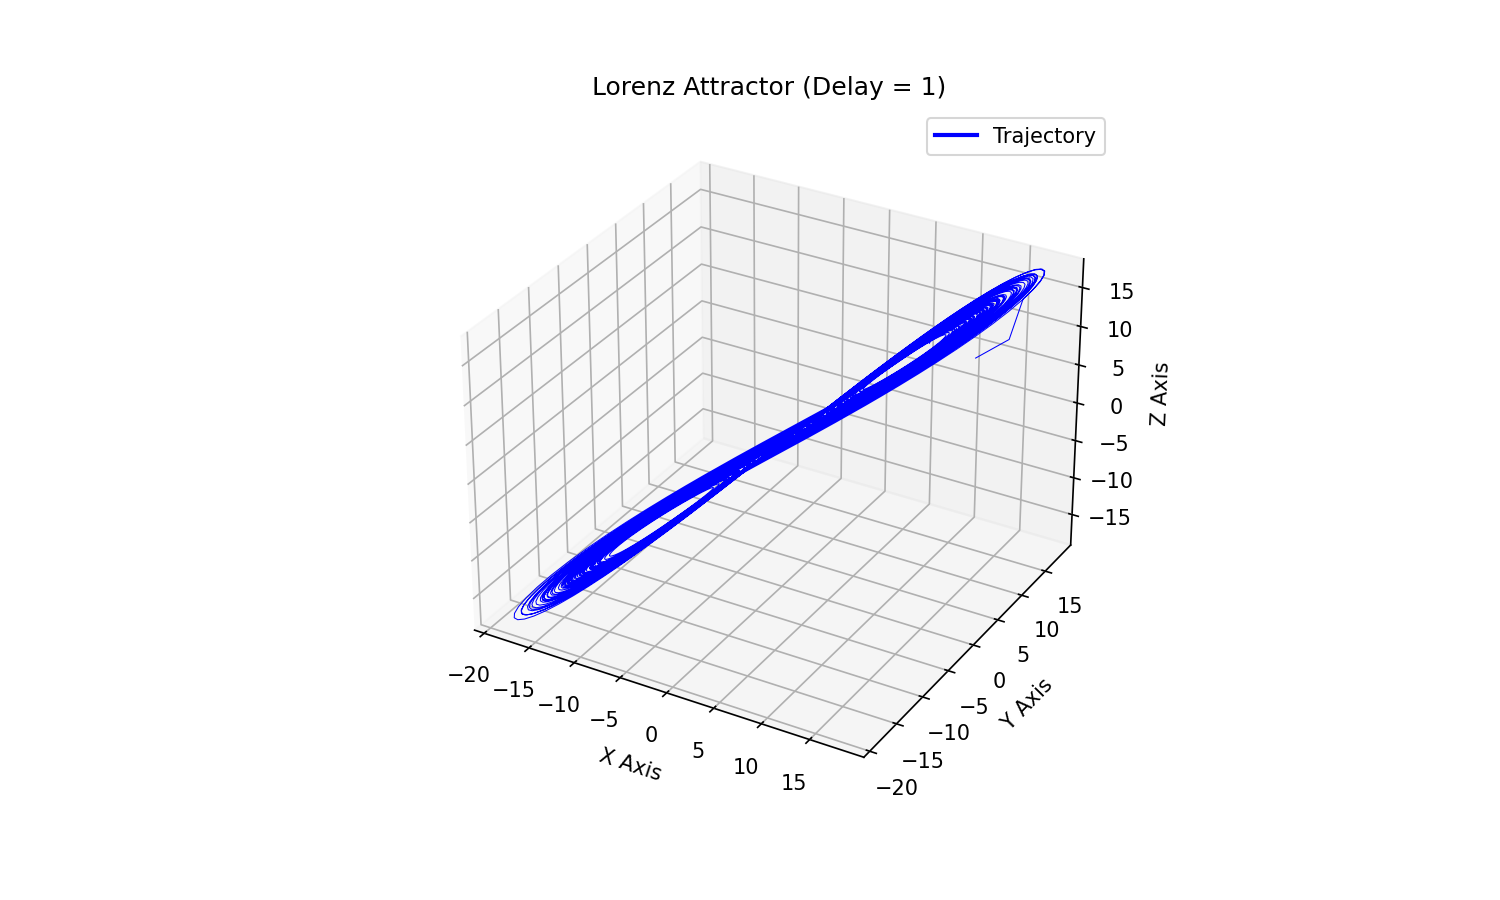
\includegraphics[width=0.45\textwidth]{images/trajectory_lorentz_1.png}\label{lorenzdelaya}}
\subfigure[Delay = 20]{
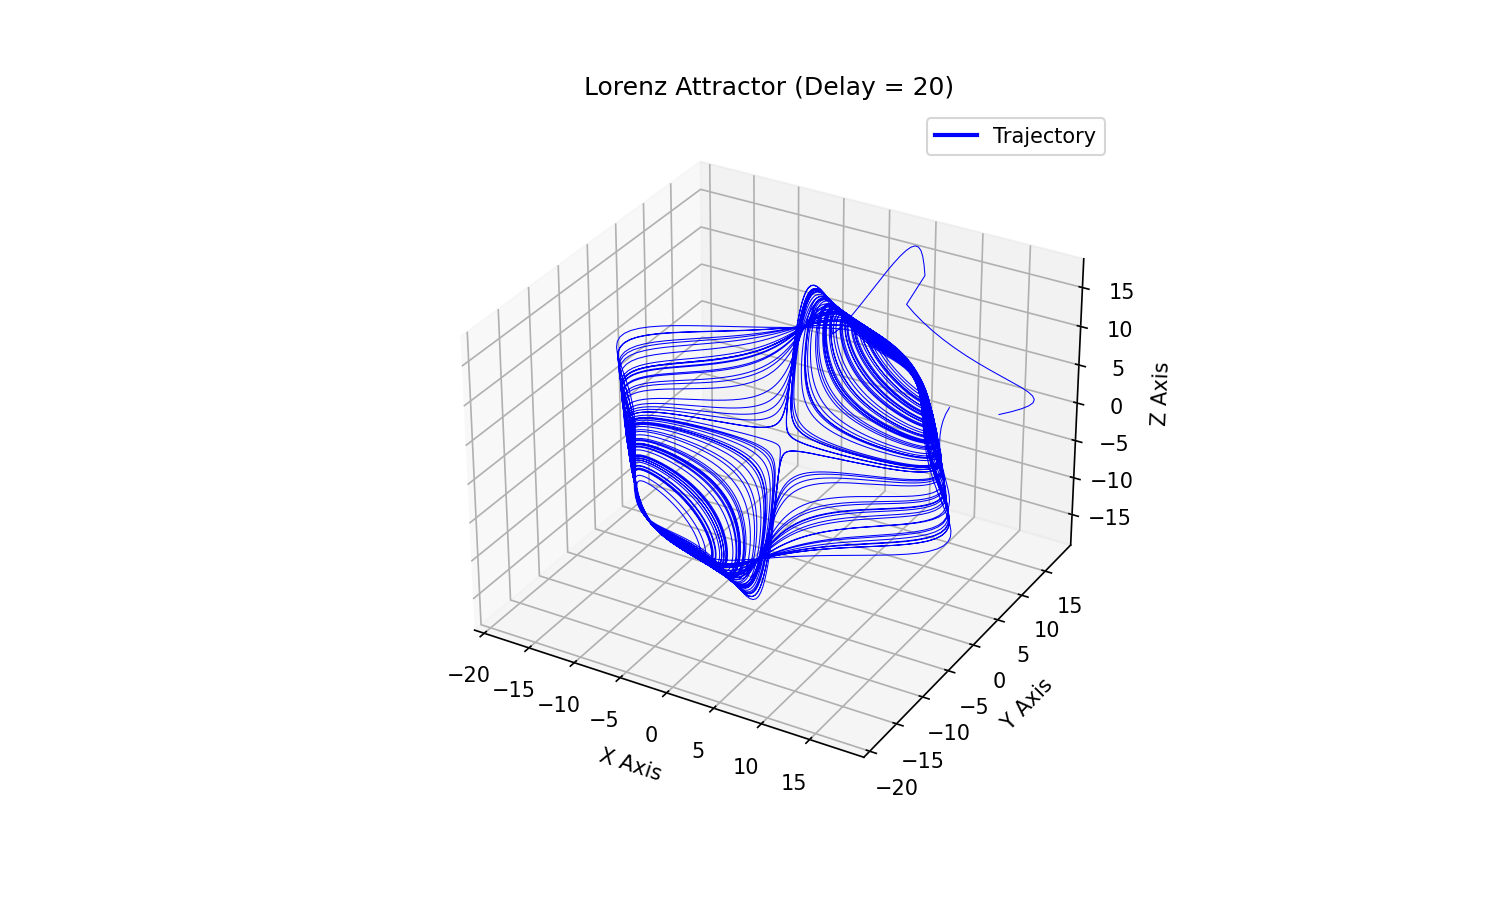
\includegraphics[width=0.45\textwidth]{images/trajectory_lorentz_20.png}\label{lorenzdelayb}}
\subfigure[Delay = 200]{
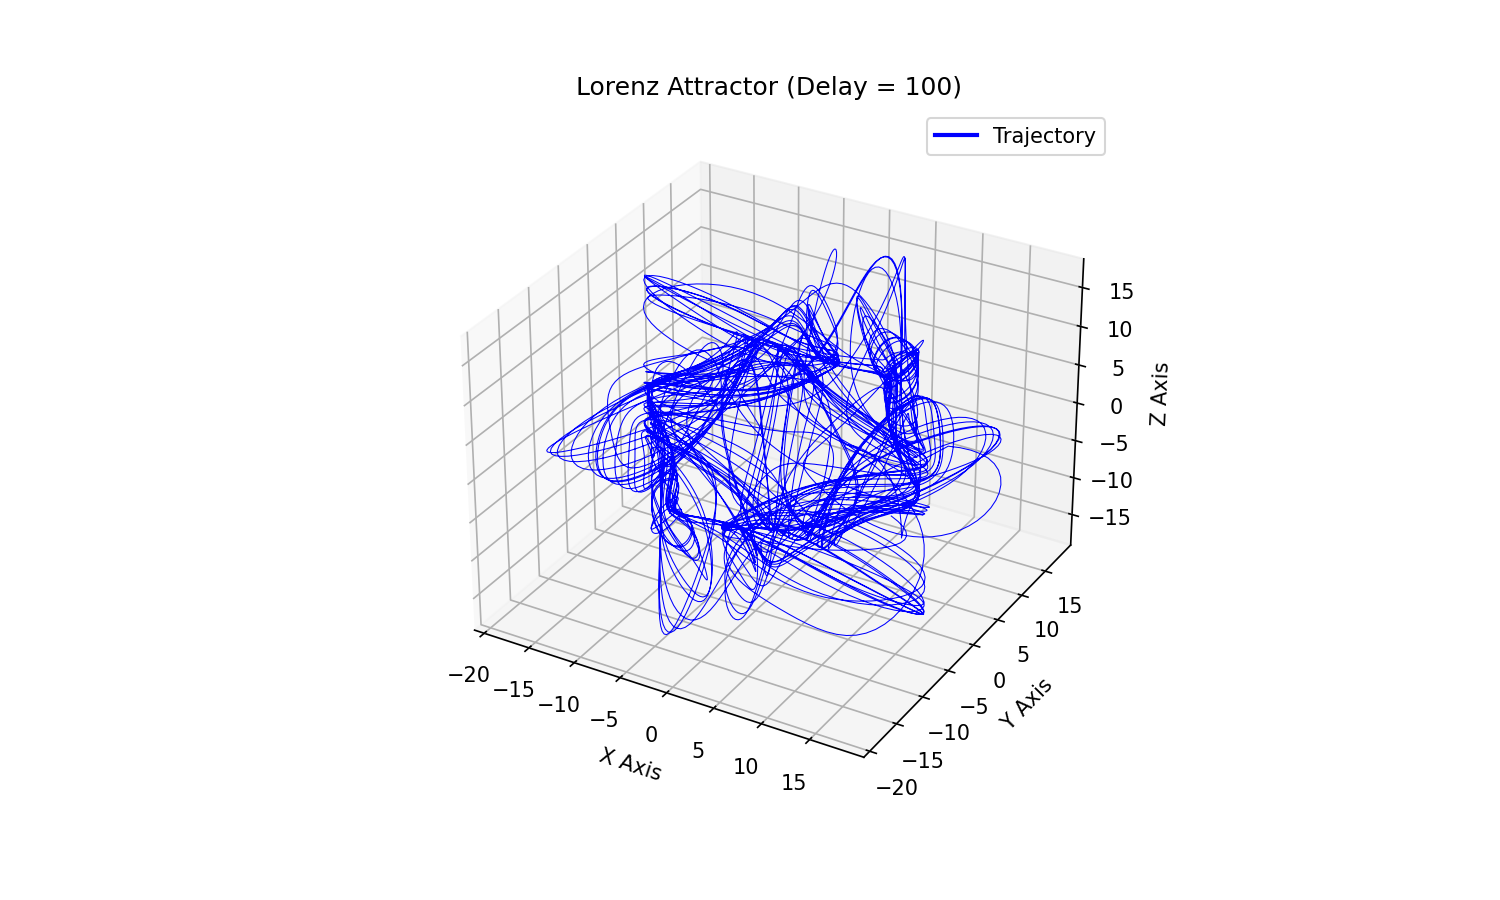
\includegraphics[width=0.45\textwidth]{images/trajectory_lorentz_100.png}\label{lorenzdelayc}}
\caption{Effect of delay in the Lorenz approximation}
\label{lorenzdelay}
\end{figure}

Using the algorithm to select the best delay value we get \(\Delta t = 7\). This aligns with our earlier hypothesis, as \(7 < 20\) and \(2\Delta t = 14 < 20\). Therefore, none of the delayed vectors are yet chaotic with respect to the original vector. As we can see in Figure \ref{lorenzbest} the shape of the attractor can be approximated in a correct way, allowing us to get an intuition of the system behaviour only using the x-coordinate.
\begin{figure}[H]
\centering
\subfigure[3D plot]{
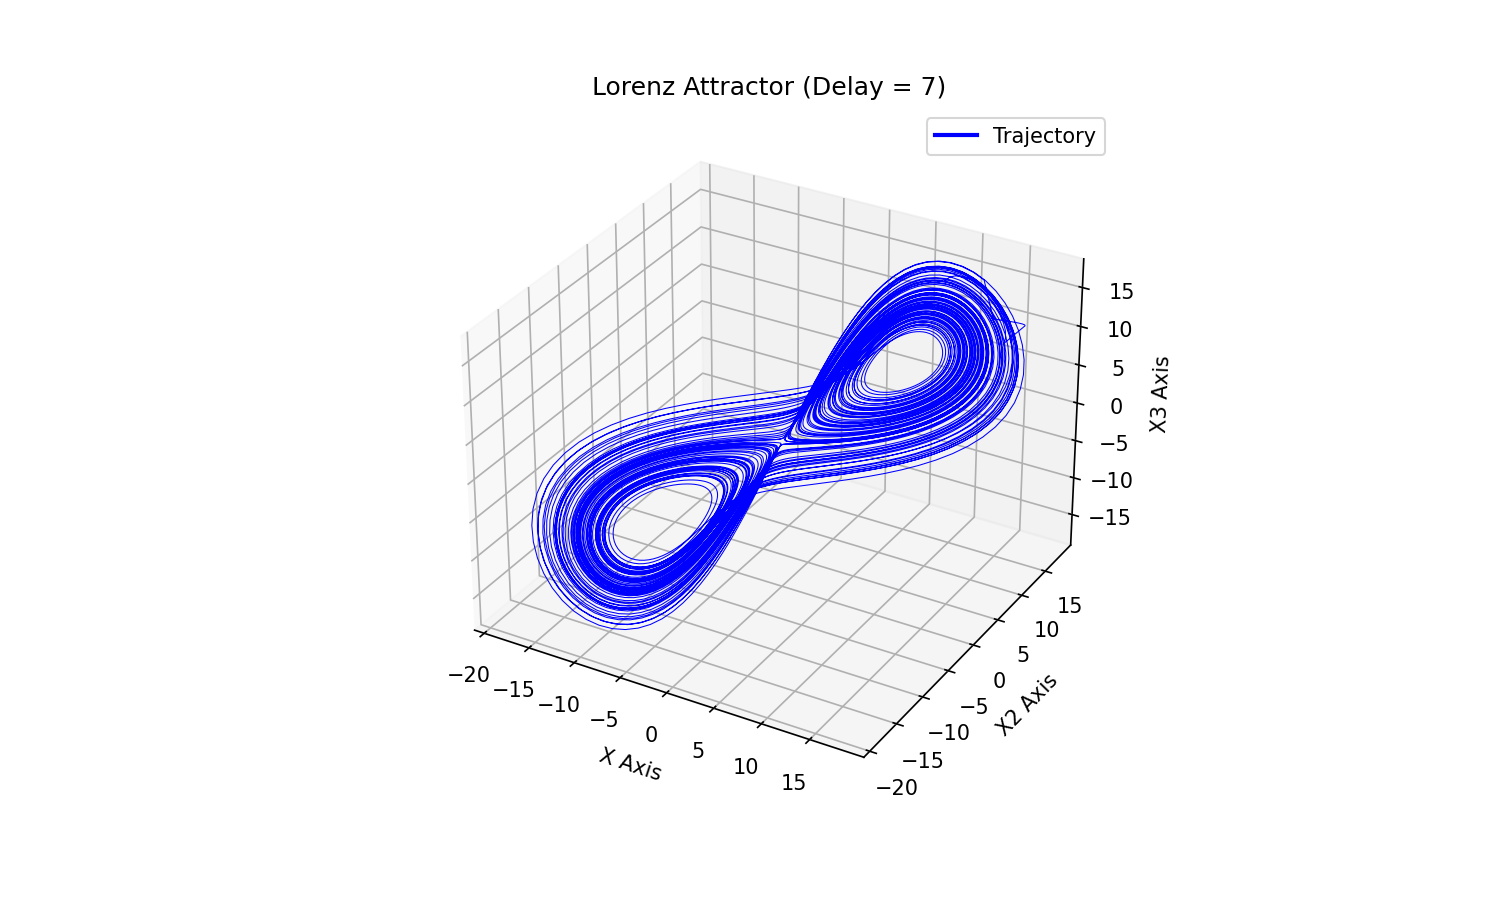
\includegraphics[width=0.6\textwidth]{images/trajectory_lorentz_best.png}\label{lorenzbesta}}
\subfigure[XZ planes plot]{
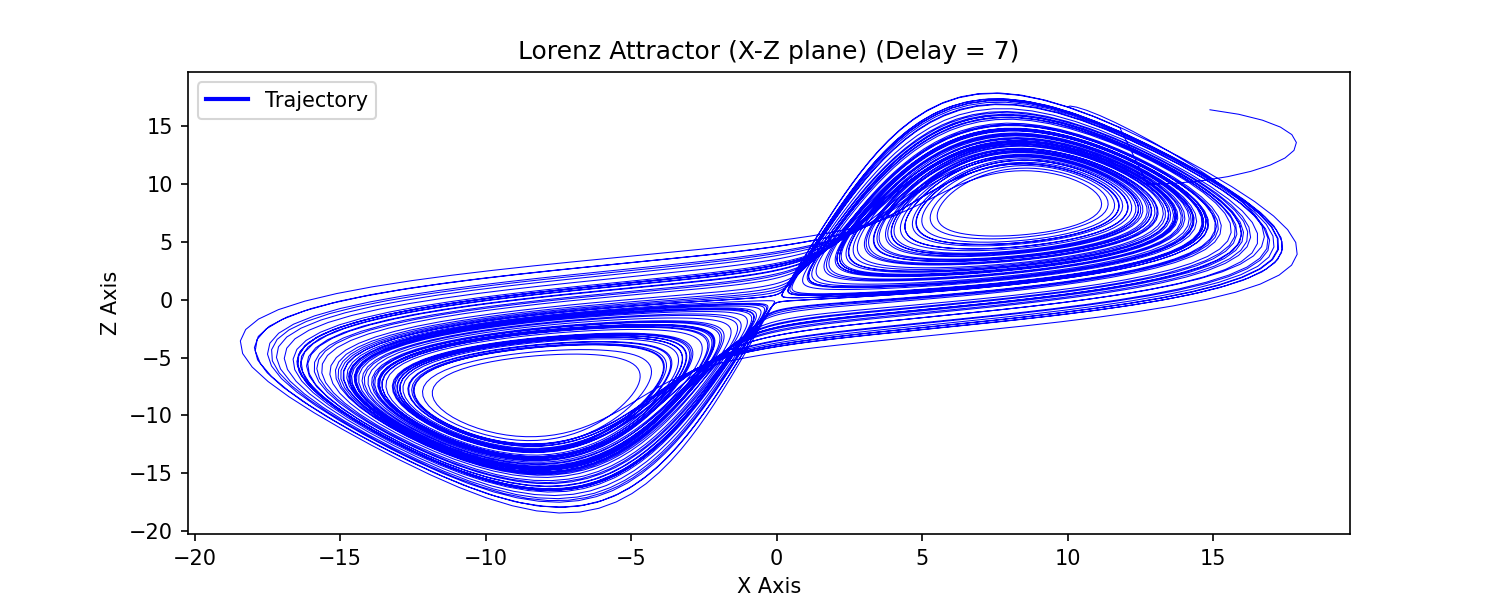
\includegraphics[width=0.45\textwidth]{images/trajectory_lorentz_xz_best.png}\label{lorenzbestb}}
\subfigure[Distance for each value of \(\Delta t\) to the original trajectory]{
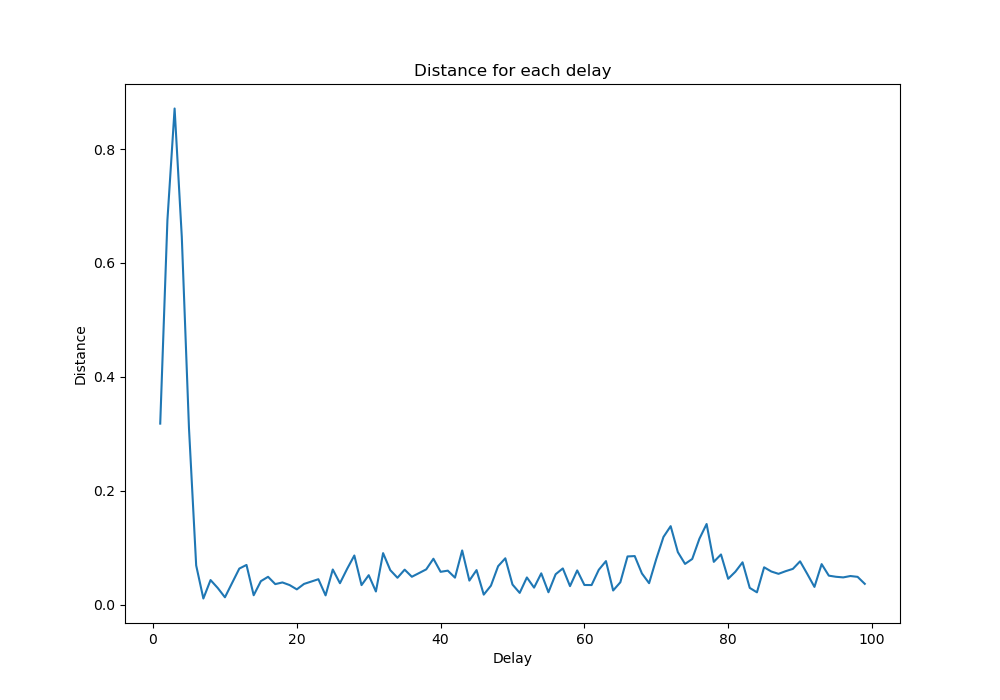
\includegraphics[width=0.45\textwidth]{images/distance.png}\label{lorenzbestc}}
\caption{Lorenz approximation}
\label{lorenzbest}
\end{figure}
An intriguing observation is that the algorithm computes a similar distance for values of \(\Delta t\) such as 20 or 100 (Figure \ref{lorenzbestc}, even though we observed that their shapes differ significantly from the real trajectory. This phenomenon may be attributed to the inherent chaotic nature of the system as well as the distance being composed of small peaks and valleys rather than a straight, linear relationship. Also, already in the previous Exercise we observed that, in spite of two Lorenz systems being very similar in structure, their trajectories differed greatly when the distance between them was measured. Therefore, the euclidean distance may not be the best method to obtain the delay overall.

\begin{figure}[H]
\centering
\subfigure[3D plot]{
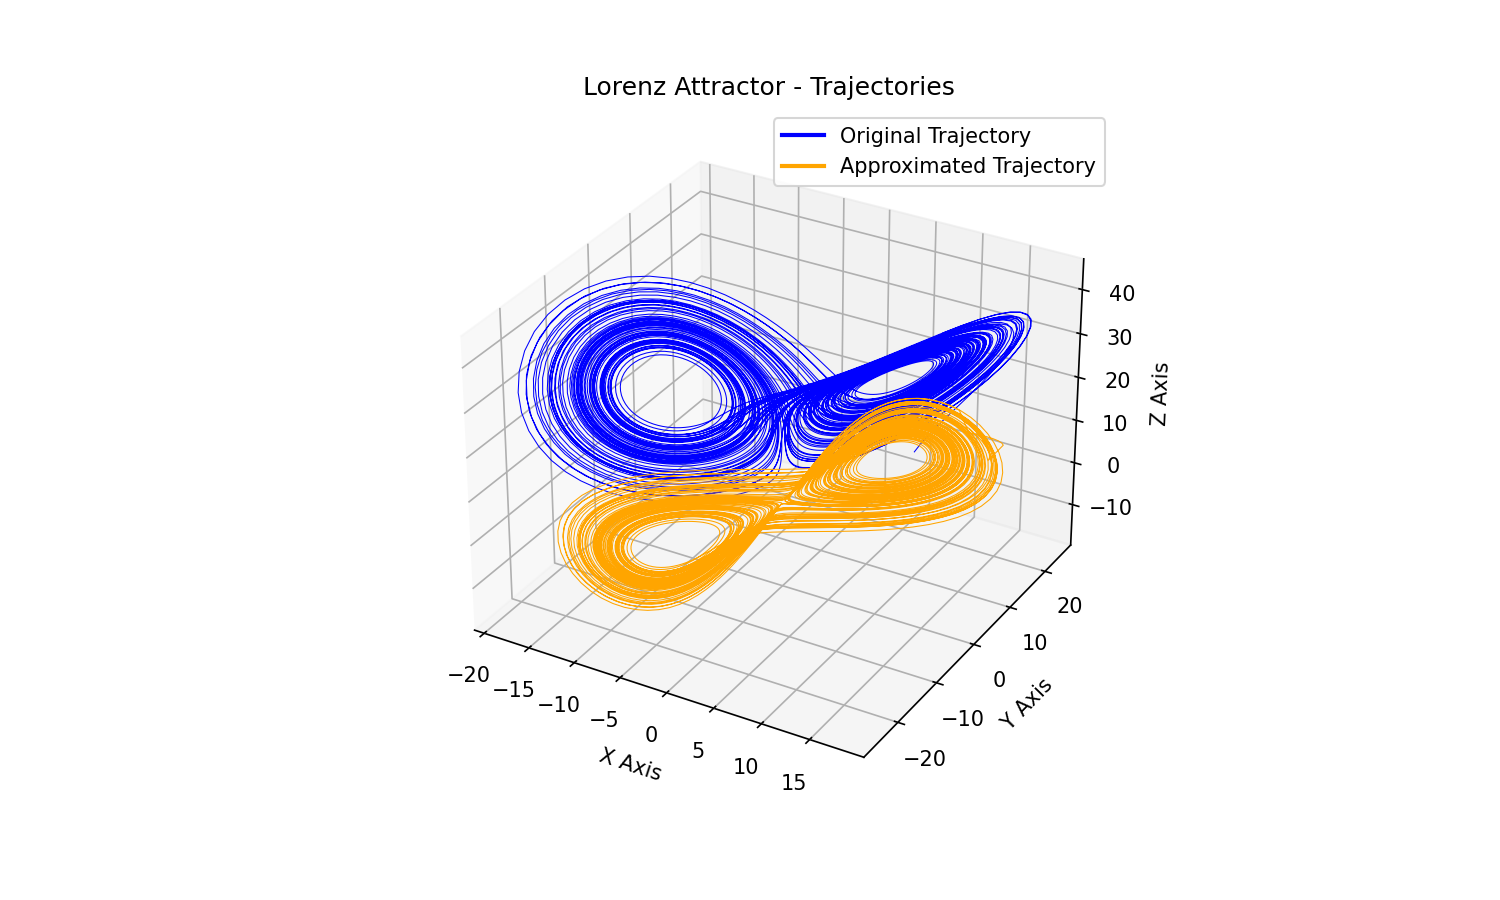
\includegraphics[width=0.6\textwidth]{images/trajectory_lorentz_mul.png}\label{lorenzcompa}}
\subfigure[XZ planes plot]{
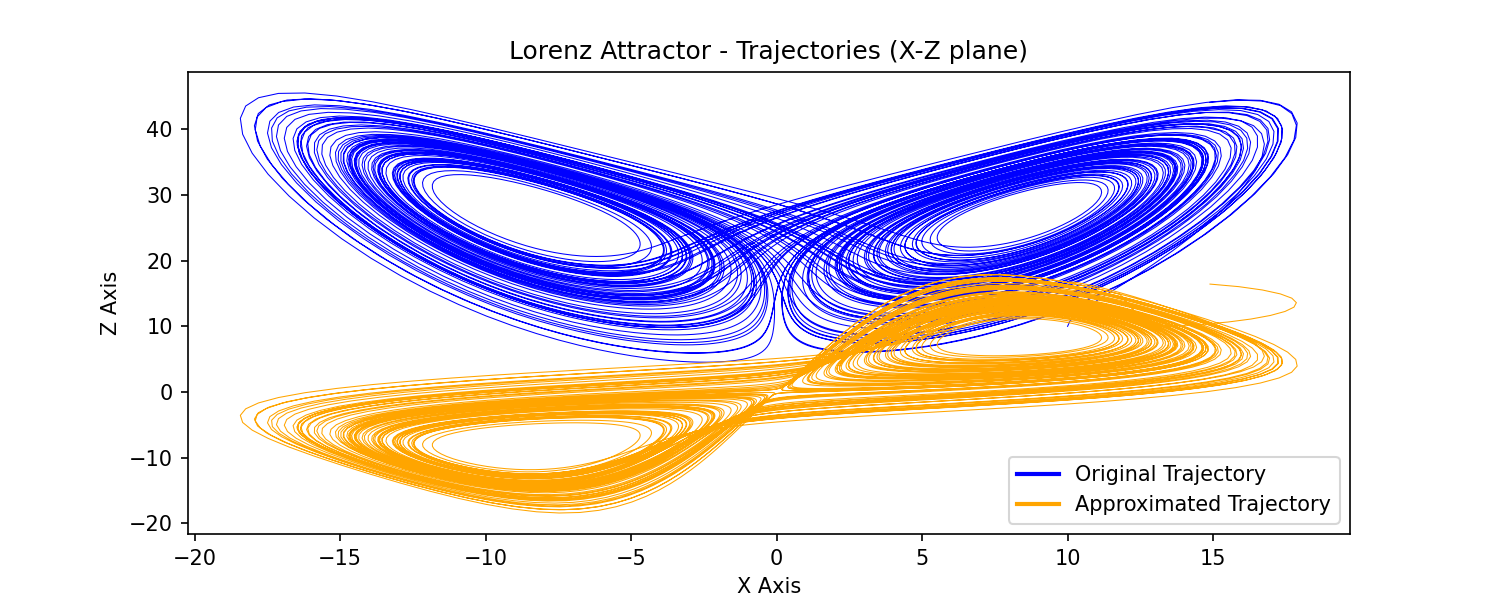
\includegraphics[width=0.5\textwidth]{images/trajectory_lorentz_mul_xz.png}\label{lorenzcompb}}
\caption{Comparison between the original trajectory and the approximation}
\label{lorenzcomp}
\end{figure}

In Figure \ref{lorenzcomp}, we can compare and conclude that the shape of the original system can be reasonably represented using only the x-coordinate and the delayed vectors. However, while the overall shape appears similar, a closer inspection in Figure \ref{lorenzcompa} reveals distinct differences in curvature and folding. Additionally, in Figure \ref{lorenzcompb}, we notice that the approximation is positioned at a lower value, and its shape is not completely symmetrical with respect to the line \(X=0\) as seen in the original shape. 

In Part 2 of this task, it's important to note that we haven't excluded the last \(delay\) rows when plotting. Now, we have much more data and therefore the plot is barely affected by it, as we can see in Figure \ref{lorenzskip}. The only thing that changes compared to Figure \ref{lorenzbestb} in the plot is a little trajectory in the upper-right corner.
\begin{figure}[H]
\centering
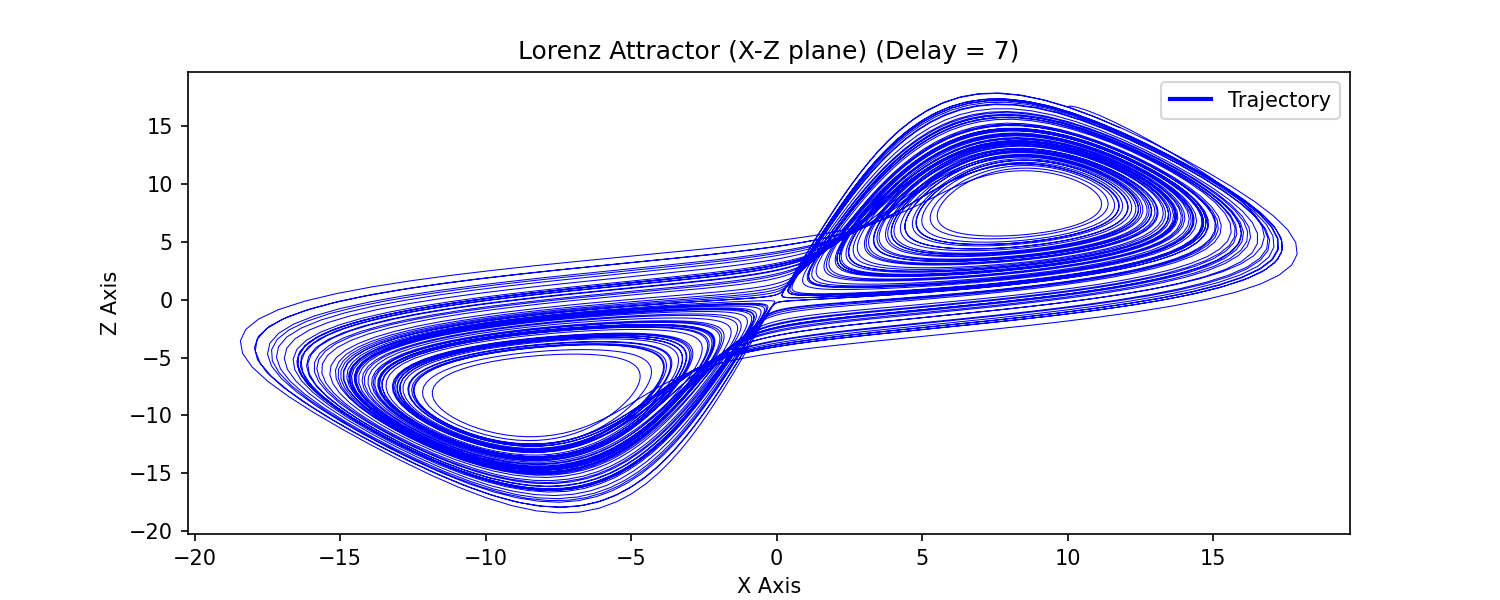
\includegraphics[width=0.5\textwidth]{images/trajectory_lorentz_xz_skip.png}
\caption{Approximation of Lorenz system skipping the last \(delay\) rows}
\label{lorenzskip}
\end{figure}



Finally, we can try to approximate the Lorenz system using only the z-coordinate now, applying the same method as before. However, we can note in the results obtained in Figure \ref{lorenzz} that the approximation does not resemble the original shape.
\begin{figure}[H]
\centering
\subfigure[3D plot]{
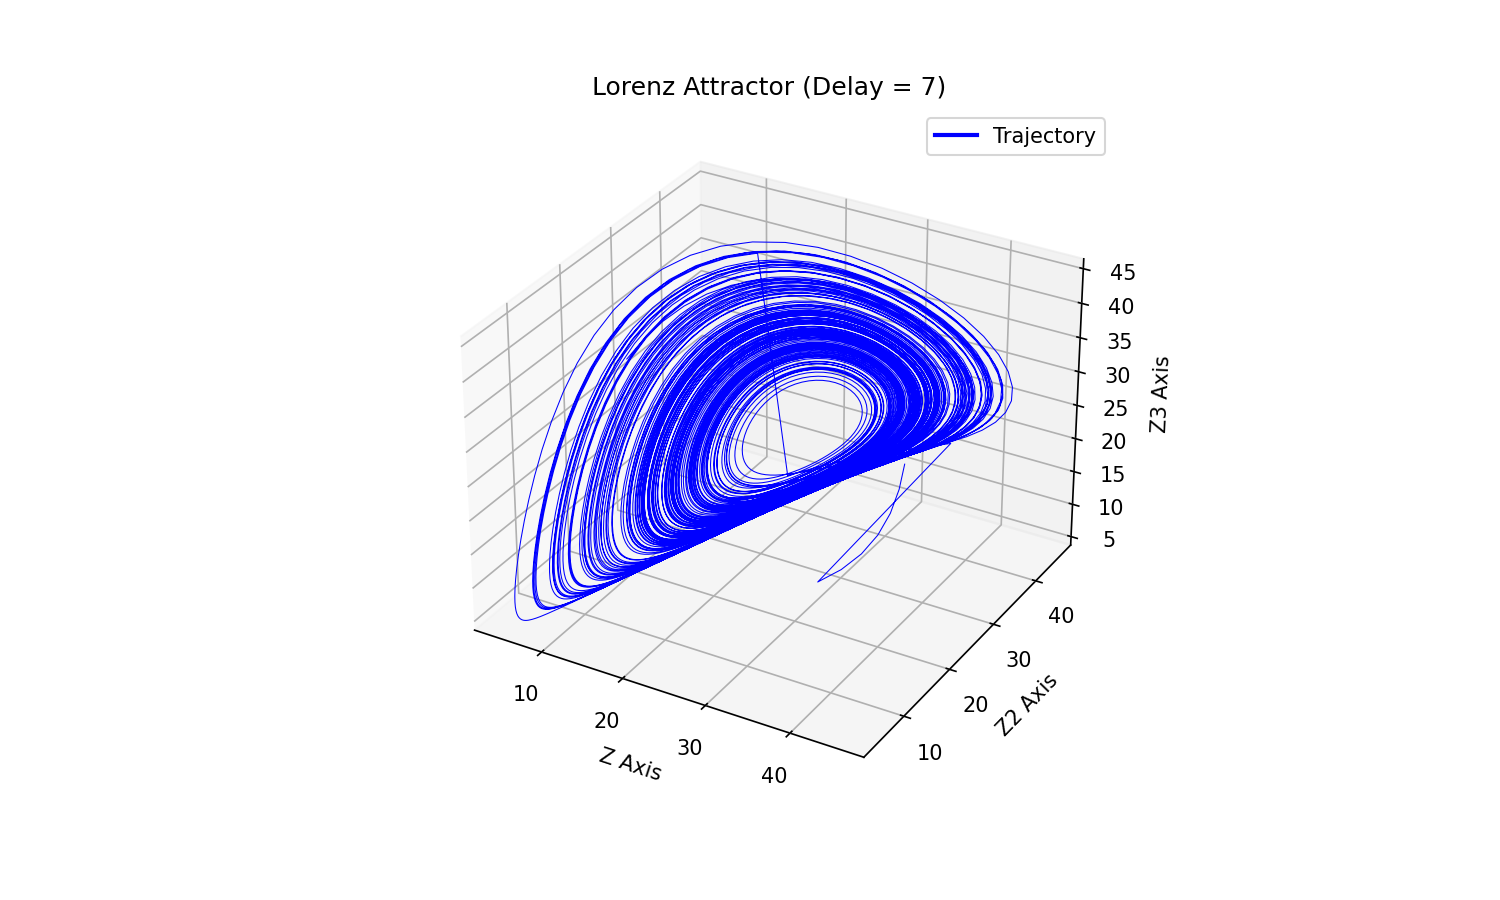
\includegraphics[width=0.6\textwidth]{images/trajectory_lorentz_Z.png}\label{lorenzza}}
\subfigure[XZ planes plot]{
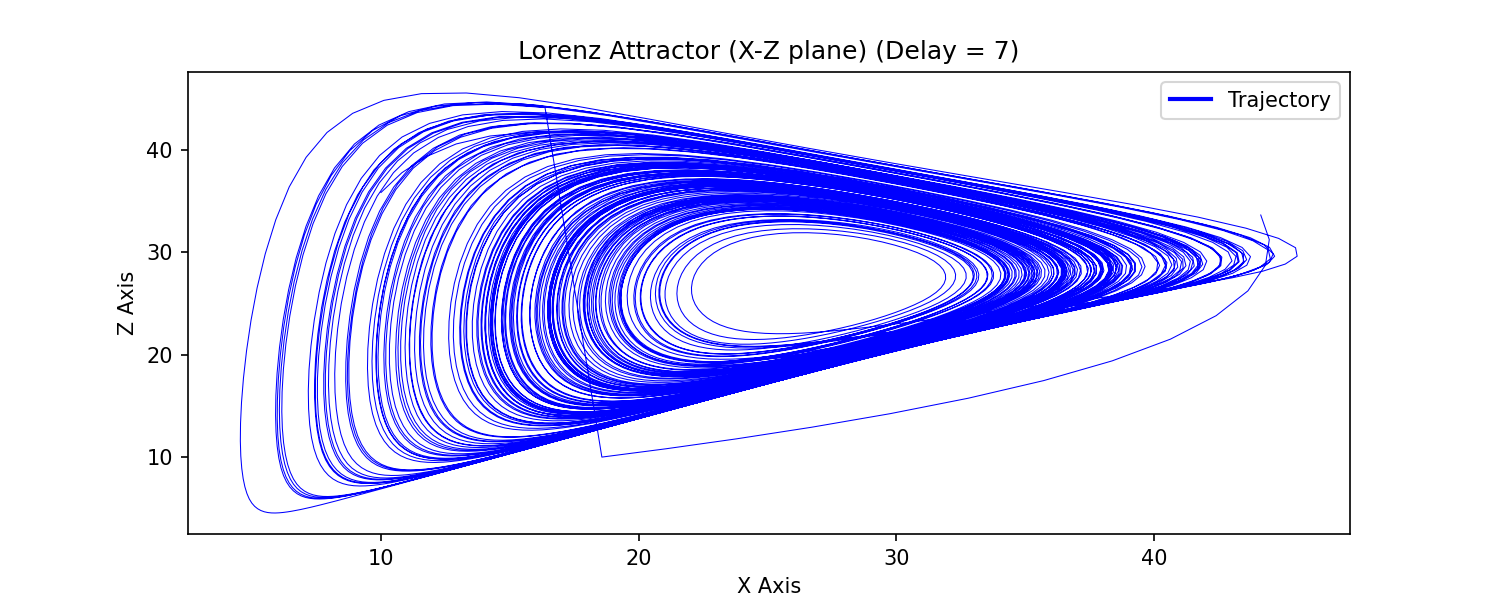
\includegraphics[width=0.5\textwidth]{images/trajectory_lorentz_xz_z.png}\label{lorenzzb}}
\caption{Approximation of the Lorenz system using z-coordinate}
\label{lorenzz}
\end{figure}

One possible explanation for this phenomenon is that the x and y coordinates may be more informative than the z coordinate. Consequently, attempting to reconstruct the system using the z coordinate becomes more difficult. On the other hand, the parameters \(\rho = 28\) and \(\beta = 8/3\) may play a role, particularly in their impact on z through \(\rho - z\) and \(\beta z\), making z less influential in the system.

Nevertheless, we can try to go even deeper, first reminding the system of equations that rule the Lorenz attractor:
\begin{align*}
\frac{dx}{dt} &= \sigma (y - x) \\
\frac{dy}{dt} &= x (\rho - z) - y \\
\frac{dz}{dt} &= xy - \beta z
\end{align*}

Analyzing the system we can note that z is determined by \(xy\) minus a multiple of z. However, we can notice that z is indeed loosing information, as its value is the same when we have \((x(t),y(t))\) and \((-x(t), -y(t))\), as in the z formula both minus signs are cancelled. Therefore, we can assert that z is less informative than x and y due to its lack of sensitivity to the sign of the solution. This lack of uniqueness in the mapping of z may prevent a clear reconstruction of the original solution when only the z-coordinate is considered. This assertion finds backing in a visual criterion: the z representation closely resembles one of the symmetric halves that form the Lorenz attractor. Then, we can hypothesize that the results of Figure \ref{lorenzz} might be illustrating a collapsed solution between the original trajectory and the sign-reversed trajectory, of which z cannot distinguish and therefore, properly represent. 
\end{task}